\section{Introduction}\label{section introduction}


{\bf Context.} 
Resilience is a key notion for improving safety of unperfect systems and resilience engineering is a paradigm for safety management that focuses on systems coping with complexity and balancing productivity with safety (\cite{challenges} analyse 472 contributions in this domain). Some systems are subjects at frequent intervals to accidents, attacks or changes. Think for instance of a supply chain, or an airport’s air trafic control. In such cases, a question that arises is that of whether the system can return to its normal (safe) behavior after an accident or attack [pushed it towards some kind of ‘error state’] and, if it can, whether it can perform the return in a satisfactory timeframe. In the exemple of air trafic control, an accident i.e. for instance a delay in the arrival of a plance can lead to conflicts of resolution (i.e. landing) which lead to prompting planes to remain on standby. Since their fuel quantity is limited it is hence pretty important to be able to know that trafic will return to its normal pace quickly enough. This is the resilience problem. 
Resilience is the capacity of a system that fall in a bad set of states to leave this set and to reach a safe set of states.

%
%{\bf MFCS 2023
%Abstract submission deadline:    	 April 24th (AoE) 
%Paper submission deadline:    	April 28th (AoE)} \\
%%
%{\bf CONCUR 2023 Abstract Registration Due 	Apr 24, 2023
%Submission Deadline 	May 2, 2023}\\

{\bf FSTTCS 2033  Submission deadline: July 14, 2022 AoE (firm)
Notification to authors: September 16, 2022}

trop d'hypotheses trop fortes sur les WSTS

{\bf Our contributions}

\begin{itemize}

\item We introduce a general definition of resilience extending the state-resilience \cite{DBLP:journals/corr/PrasadZ16,DBLP:journals/corr/abs-2108-00889,DBLP:conf/gg/Ozkan22} and we define three decidability questions for each of type of resilience: The (state-)resilience problem (RP), the bounded (state-)resilience problem (BRP)
and the $k$-(state-)resilience problem (kRP). The (general) resilience problem is the following: let $L_1,L_2 \subseteq S$ be two subsets of states, S is $(L_1,L_2)$-resilient if $\post^*(L_1)	\subseteq \pred^*(L_2)$. We remark that it is an instance of the home space problem defined in the framework of VASS in \cite{DBLP:journals/corr/abs-2207-02697}.
State-resilience (called resilience in \cite{DBLP:journals/corr/PrasadZ16,DBLP:journals/corr/abs-2108-00889,DBLP:conf/gg/Ozkan22}) is ...

\item Surprinsingly, the general undecidability statements were not known neither proved. We show that resilience and state-resilience problems are both undecidable for WSTS with strong compatibility. 

%\item safe clos haut, bad clos par le bas: resilience = reachability d'un clos par le bas (anti-coverability)

\item We find classes of WSTS that have a \emph{decidable} resilience. The resilience problem (RP), the bounded resilience problem (BRP)
and the $k$-resilience problem (kRP) are decidable for completion-post-effective $\omega^2$-WSTS with strong compatibility and two sets $\Bad = \downarrow \Bad$ and $\Safe = \uparrow \Safe$.

\item The resilience problem is decidable for ideal-effective WSTS with 
$\Safe=\downarrow \Safe$
and $\Bad=\uparrow \Bad$
and
the additional hypothesis that
for all downward-closed set $D \subseteq S$, the set $\pred^*(D)$ is downward-closed.

\item Unfortunately, {\sc State-resilience},
{\sc Bounded-state-resilience} and
{\sc $k$-state-resilience}
are undecidable for strongly upward-compatible WSTS with effective pred-basis
when
$\Safe=\uparrow \Safe$
and $\Bad=\downarrow \Bad$. We made a reduction of zero-reachability in reset-VASS to state-resilience in reset-VASS that are WSTS with strong upward-compatibility and with effective pred-basis.

\item We generalize the main theorem of \cite{} by relaxing the strong compatibility hypothesis: {\sc State-resilience} is decidable for 
 WSTS with effective 
$\uparrow$ $\post^*$ basis
when
$\Safe=\uparrow \Safe$
and $\Bad=\downarrow \Bad$. However, we show that removing the effective 
$\uparrow$ $\post^*$ basis hypothesis leads to undecidability. But we found another effective hypothesis {\sc State-resilience} is decidable for ideal-effective WSTS with downward and upward compatibilities. and {\sc $k$-state-resilience} and {\sc bounded-state-resilience} are decidable for ideal-effective WSTS with strong downward compatibility.

\item We study the resilience for VASS and most of problems are shown decidable.
\end{itemize}


{\bf Related works.} 
In 2016, Prasad and Zuck introduced rather informally \cite{DBLP:journals/corr/PrasadZ16}, the state-resilience of a process to an adversary and they used the framework of WSTS enjoying \emph{both} upward and downward compatibilities to shortly draw a proof of the decidability of two kinds of resilience. Remark that the downward compatibility of a WSTS implies  there exists an algorithm that computes a finite basis of $\uparrow \post^*(s)$ for all state $s$. In 2021 and 2022, Okzan and Würdemann \cite{DBLP:journals/corr/abs-2108-00889,DBLP:conf/gg/Ozkan22} studied graph transformation systems and they considered the state-resilience in the framework of WSTS with strong compatibility and with the supplementary hypothesis that there exists an algorithm that computes a finite basis of $\uparrow \post^*(s)$ for all state $s$. All these papers consider particular Safe and Bad sets: $\Bad$ is downward-closed and $\Safe$ is upward-closed.
 



\begin{center}
	\begin{figure}
			\hspace{0.75cm}
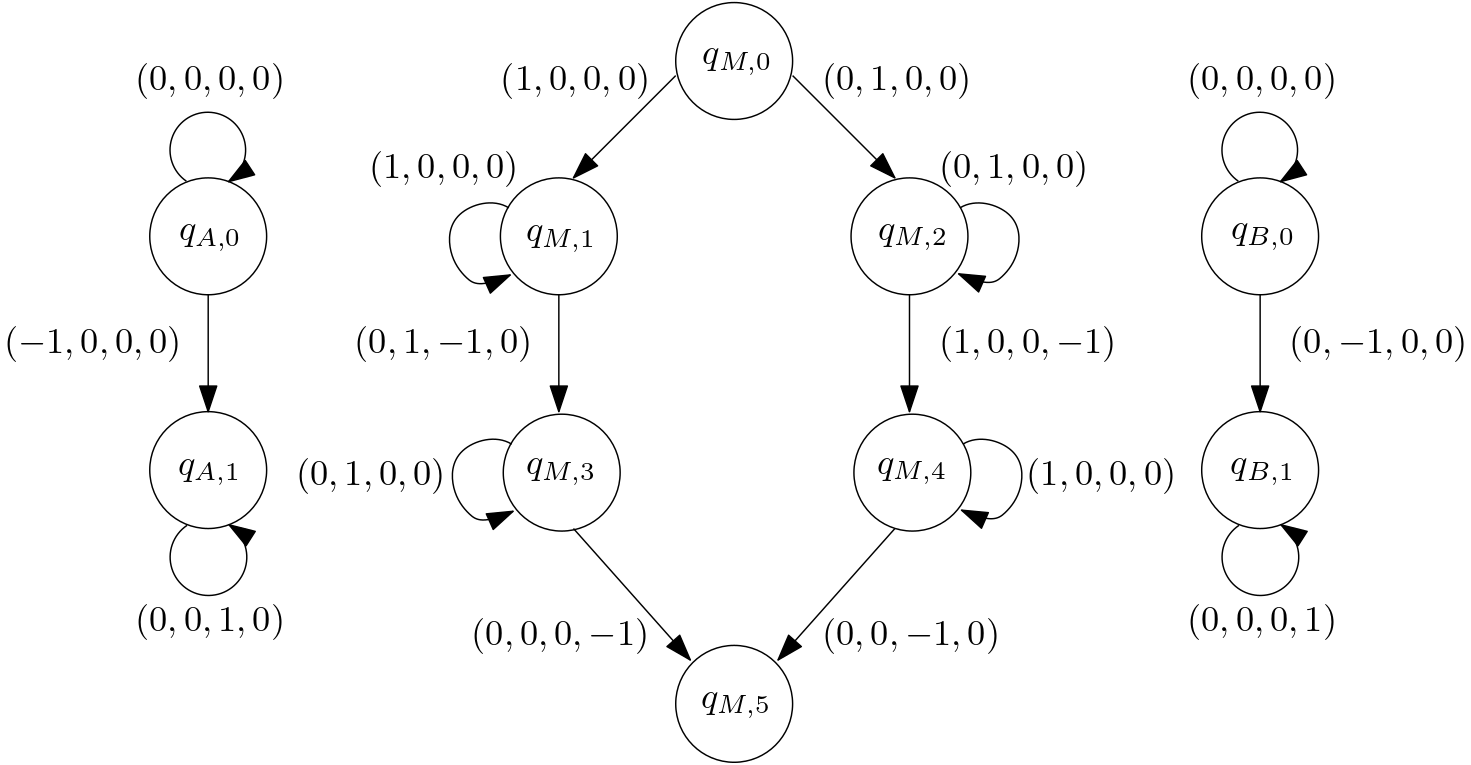
\includegraphics[width=0.85\textwidth]{FigureB}
	\caption{A channel system with three automata and four channels. Leftmost and rightmost automata represents aircrafts attempting to land and staying on stand-by in the air while they haven't received permission to land, while the middle one represent the control tower managing the aircrafts landings so that only one aircraft at a time is allowed for landing.}
					\label{air control}
	\end{figure}
\end{center}

Consider the channel system in Figure~\ref{air control}. It models a scenario in which two aircrafts wants to land in an airport at the same time. 

The automata on the left and right represents the aircrafts attempting to land, while the middle one represent the control tower. The control tower can send messages to the aircrafts using channels $c_1$ and $c_2$, and these in turn can send messages to the control tower using respectively channel $c_3$ and $c_4$. Remark channels $c_3$ and $c_4$ have a unary alphabet
in the exemple and therefore can be seen as counters. 

Safety requires that only one aircraft at a time attempt to land. The role of the control tower is to ensure this;
there are two possible choices: aircraft A waits for aircraft B to land
or vice-versa. To make its choice known to the aircrafts, the control tower will send them messages using the channels. 
We assume that the channel are
lossy \-- i.e. an arbitrary number of messages may be lost from the channels \--  but that they are still such that out of ten messages, at least one is not lost.
In this example, the safe, desirable state would be one where the aircrafts have both landed. 
Resilience here expresses that the aircrafts state will both land, while explicit resilience or $k$-resilience asks whether they will do so in at most $k$ steps. 
Explicit resilience is of interest since in general we want to ensure the safe state will
be reached in
the least amount of step possible. 
In this exemple, for instance, aircrafts cannot simply wait in the air an infinite amount of time.
With one out of ten messages guarranteed to not be lost, $40$-resilience hold in the example.

%\alain{il faut mieux expliquer le modèle, le rôle des 4 canaux, des messages, remarquer que 2 canaux sont des compteurs,....}

% contrôle de trafic aérien, perturbation dans le planning → Bad (par exemple, trop d’avions qui cherchent à atterir en même temps et qui doivent être mis en stand-by au dessus de l’aéroport?) → Safe (trafic fluide à nouveau). K-résilience important car les avions peuvent pas rester indéfiniment en stand-by (re : le carburant est un réactif limitant) 



